% Section 5 - Docker
% Roberto Masocco <roberto.masocco@uniroma2.it>
% May 17, 2023

% ### Docker ###
\section{Docker}
\graphicspath{{figs/section5/}}

% --- Docker Engine ---
\begin{frame}{Docker Engine}
	\begin{columns}
		\column{.5\textwidth}
		\textbg{Docker} is the currently de-facto standard for building, managing and distributing \textbg{multiplatform} containers.
		\newline\newline
		It is an engine (\emph{i.e.}, a collection of \textbg{daemons}) that automates the management of the kernel subsystems in order to set up, store and run containers.

		\column{.5\textwidth}
		\begin{figure}
			\centering
			\label{fig:docker}
			
\includegraphics[scale=.2]{docker.png}
			\caption{Docker logo.}
		\end{figure}
	\end{columns}
\end{frame}
\begin{frame}{Docker Engine}
	\begin{figure}
		\centering
		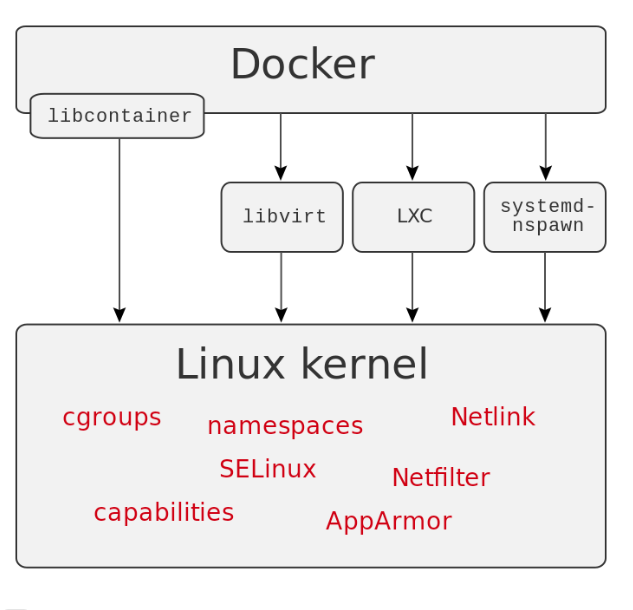
\includegraphics[scale=.29]{dockerScheme.png}
		\label{fig:dockerscheme}
		\caption{Docker Engine scheme.}
	\end{figure}
\end{frame}

% --- Containers in robotics ---
\begin{frame}{Containers in robotics}
	Containers can be of help in some classic scenarios:
	\begin{itemize}
		\item \textbg{deploying} applications or whole control architectures, solving issues like \textbg{dependencies} and \textbg{configurations};
		\item configuring and distributing \textbg{development environments};
		\item working with \textbg{multiple architectures} at the same time: Docker fully supports \href{https://www.qemu.org/}{\color{blue}\textbf{\underline{QEMU}}} to build and run containers;
		\item expanding the capabilities of \textbg{(partially) closed-source} hardware solutions (\emph{e.g.}, Nvidia Jetson...).
	\end{itemize}
\end{frame}

% --- Building a Docker container ---
\begin{frame}{Building a Docker container}{Step by step}
	\begin{enumerate}
		\item A \textbg{Dockerfile} specifies a set of rules to build an \textbg{image}, just like a script.
		\item \textbg{Images} are the binary archives from which a \textbg{container} can be started: they can be stored, pulled from a remote \textbg{registry} or simply built locally.
		\item A \textbg{container} can be built from an image and then started, stopped and managed by the Docker daemon.
		\item Processes started inside the container are subject to its limitations, \emph{e.g.}, \textbg{filesystem jails} prevent them to climb up to the hosts's filesystem.
	\end{enumerate}
	Images are built \textbg{incrementally}: each Dockerfile directive defines a new \textbg{layer}, and the Docker engine stores the differences between each build step thanks to \textbg{OverlayFS}.\\
	For every new container, its filesystem will be in a \textbg{new top layer}.\\
	This allows to efficiently \textbg{cache and share build stages}, which will then be stacked together to form images, but operating in a \textbg{copy-on-write}, \textbg{slower} fashion.
\end{frame}

% --- Dockerfiles ---
\begin{frame}[fragile]{Dockerfiles}
	\begin{columns}\column{.9\textwidth}
		\begin{lstlisting}[language=Dockerfile, caption=Minimal example of a Dockerfile running an Ubuntu image in a container.]
ARG VERSION=22.04
FROM ubuntu:$VERSION # Note the tag!

ENV DEBIAN_FRONTEND=noninteractive

RUN apt-get update && \
    apt-get install -y --no-install-recommends \
    build-essential \
    git && \
    rm -rf /var/lib/apt/lists/* /tmp/* /var/tmp/*/apt/lists/*

ENV DEBIAN_FRONTEND=dialog
LABEL maintainer.name="Roberto Masocco"
CMD ["bash"]
\end{lstlisting}
	\end{columns}
\end{frame}

% --- Dockerfile commands ---
\begin{frame}{Dockerfile commands}
	\begin{itemize}
		\item \texttt{FROM repository/image:tag}\\Specifies a base image to pull.
		\item \texttt{RUN command}\\Runs the following command in a new shell inside the container.
		\item \texttt{COPY source target}\\Copies a file into the container.
		\item \texttt{ENV variable=value}\\Sets an environment variable inside the container.
		\item \texttt{ARG name=value}\\Declares a build argument.
		\item \texttt{CMD ["command", "arg1", ...]}\\Specifies the command to run when the container is started.
	\end{itemize}
\end{frame}

% --- Docker commands ---
\begin{frame}{Docker commands}
	Again, just a few (each with a gazillion of options):
	\begin{itemize}
		\item \texttt{docker build}\\Builds a new image from a Dockerfile.
		\item \texttt{docker run}\\Builds and starts a container, optionally overriding the command (\texttt{CMD}).
		\item \texttt{docker ps}\\Lists active containers.
		\item \texttt{docker exec}\\Runs a command inside a container (\emph{e.g.}, a shell).
		\item \texttt{docker start}\\Starts a container.
	\end{itemize}
\end{frame}
\begin{frame}{Docker commands}
	\begin{itemize}
		\item \texttt{docker stop}\\Stops a container.
		\item \texttt{docker images}\\Lists available images.
		\item \texttt{docker rm}\\Removes a container.
		\item \texttt{docker rmi}\\Removes an image.
	\end{itemize}
	Containers and images are usually referenced by their \textbg{ID} (\emph{e.g.}, \texttt{abae6cae4648}).
	\newline\newline
	See the \href{https://docs.docker.com/engine/reference/builder/}{\color{blue}\underline{Dockerfile reference}} and the \href{https://docs.docker.com/engine/reference/commandline/docker/}{\color{blue}\underline{Docker CLI reference}} for more.
\end{frame}

% --- Containers on real robots ---
\begin{frame}{Containers on real robots}{Best practices}
  To run containers on embedded systems and robot SBCs, some configurations are suggested which \textbg{would not apply} in traditional containerization scenarios:
  \begin{itemize}
    \item the host \textbg{network stack} should be fully exposed to allow for \textbg{ROS} and other network-based \textbg{middleware} to work properly (\texttt{-{}-network host});
    \item the \textbg{IPC namespace} should be shared to allow for \textbg{shared memory} and \textbg{IPC} to work properly (\texttt{-{}-ipc host});
    \item to allow access to the \textbg{hardware} mounted on the host, one should grant full privileges to the container (\texttt{-{}-privileged}) and mount \texttt{/dev} and \texttt{/sys} inside it (\texttt{-v /dev:/dev -v /sys:/sys});
    \item your development directory should be \textbg{mounted as a volume} inside the container, so that file manipulations happen on the host filesystem (\texttt{-v /your/code:/workspace}).
  \end{itemize}
  We would like some utility to \textbg{automate} this process...
\end{frame}
